\documentclass[a4paper, 12pt]{article}
\usepackage[T1]{fontenc}
\usepackage{lmodern}
\usepackage{color}
\usepackage{amsfonts}
\usepackage{epstopdf}
\usepackage{matlab}
%\documentclass{book}
\usepackage{blindtext}
\usepackage{hyperref}
\usepackage[brazil]{babel}
\usepackage{amssymb}
\usepackage[utf8]{inputenc}
\usepackage{amsmath}
\usepackage{indentfirst}
\usepackage{graphicx}
\usepackage{multicol,lipsum}
\usepackage[a4paper,
top=3cm, left=3cm, bottom=3cm, right=3cm]{geometry}
\usepackage{setspace}
\usepackage{multirow}
\usepackage{float}
\usepackage[dvipsnames]{xcolor}
\usepackage[table]{xcolor}
%\usepackage{pdflscape}
\usepackage[DIV=15]{typearea}
\usepackage[nottoc]{tocbibind}
\usepackage[sort,numbers]{natbib}
%\usepackage{cite}
\usepackage{matlab}

\usepackage[utf8]{inputenc}
\usepackage[T1]{fontenc}
\usepackage{lmodern}
\usepackage{graphicx}
\usepackage{color}
\usepackage{hyperref}
\usepackage{amsmath}
\usepackage{amsfonts}
\usepackage{epstopdf}
\usepackage[table]{xcolor}
\usepackage{matlab}


\documentclass[letterpaper]{article}
% bib pack %%%%%%%%%%%%%%%%%%%%%%%%%%%%%%%%%%%%%%%%%%%%%%%%%%%%%%%%%%%%%%%%%%%%%
\usepackage[utf8]{inputenc}
\usepackage{geometry}
    \geometry{left=3cm,right=2cm,top=2cm,bottom=2cm}
%
\usepackage[spanish]{babel}
%
\usepackage[fixlanguage]{babelbib}
    \bibliographystyle{babunsrt}
%
\usepackage{url}

\begin{document}
%\maketitle

\begin{titlepage}
	\begin{center}
		

\vspace{10pt}
%\begin{figure}[H][!ht]
%\centering
%
\includegraphics{puc-rio-logo.png}

%\end{figure}
\begin{figure}[!ht]
\centering

\includegraphics{images/puc-rio-logo.png}
\end{figure}
\huge{Dinâmica de Sistemas}
        \vspace{70pt}
        
		\textbf{ENG1730}
		\textbf{\large{\\ }}
		
		\vspace{30pt}
		\textbf{\small{\\Lista 05}}
		\vspace{75pt}
		
	\end{center}
	
	\begin{flushleft}
		\begin{tabbing}
			Aluno(a)\qquad\qquad\=\>Paloma Fernanda Loureiro Sette - 1621595\\
			
			Professor(a)\>João Carlos Virgolino Soares\\
	\end{tabbing}
		  
	\end{flushleft}
	\begin{center}
		%\vspace{\fill}
		\vspace{215pt}
		Rio de Janeiro, 04 de Outubro de 2022
	\end{center}
\end{titlepage}
%%%%%%%%%%%%%%%%%%%%%%%%%%%%%%%%%%%%%%%%%%%%%%%%%%%%%%%%%%%
\newpage
\tableofcontents
\thispagestyle{empty}

\newpage
\pagenumbering{arabic}

\newpage

%\newcommand{\listequationsname}{Lista de Equações}
%\newlistof{myequations}{equ}{\listequationsname}
%\newcommand{\myequations}[1]{%
%\addcontentsline{equ}{myequations}{\protect\numberline{\theequation}#1}\par}

%\listofmyequations
\newpage


\newpage

\listoffigures
\thispagestyle{empty}

\newpage
%%%%%%%%%%%%%%%%%%%%%%%%%%%%%%%%%%%%%%%%%%%%%%%%%%%%%%%%%
%%%%%%%%%%%%%%%%%%%%%%%%%%%%%%%%%%%%%%%%%%%%%%%%%%%

\newpage

\thispagestyle{empty}

\newpage

\section{Introdução}
Este relatório refere-se ao quinto trabalho da disciplina de Dinâmica de Sistemas, ENG1730, de 2022.2. Trataremos da modelagem de um sistema composto por um carro contendo um pêndulo simples, mola e amortecedor.

\section{Questão 01}
A figura a seguir mostra uma haste de massa m acoplada a uma base móvel de massa $M$. A base está atrelada a uma mola de constante $k_T$ e a um amortecedor de constante $b_T$. O eixo de rotação entre o pêndulo e a base possui atrito viscoso de coeficiente $b_R$ e uma rigidez rotacional $k_{R}$.

\begin{figure}[H]
\centering

\includegraphics[scale = 0.7]{images/sistema.png}
\label{filtro1}
\caption{Carro contendo o pêndulo simples, mola e amortecedor}
\end{figure}

As dimensões da haste são:

\begin{figure}[H]
\centering
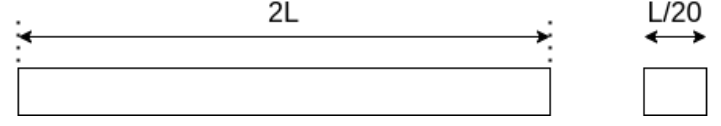
\includegraphics[scale = 0.7]{images/dim_haste.png}
\label{filtro1}
\caption{Dimensões da haste}
\end{figure}

Devemos resolver os itens propostos, organizados em tópicos a seguir.


\subsection{Modelo matemático do sistema}

Antes de começarmos a modelar o sistema, é interessante analisarmos o diagrama de corpo livre, tanto da haste quanto do carro. 

\begin{figure}[H]
\centering
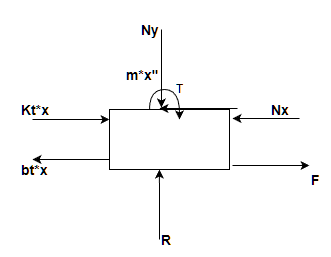
\includegraphics[scale = 0.95]{images/dcl_carro.png}
\label{filtro1}
\caption{Diagrama de Corpo Livre do carro}
\end{figure}

\begin{figure}[H]
\centering
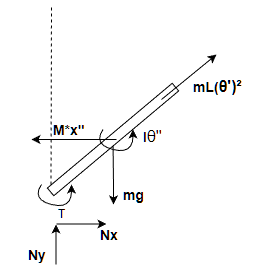
\includegraphics[scale = 0.95]{images/dcl_haste.png}
\label{filtro1}
\caption{Diagrama de Corpo Livre da haste}
\end{figure}


Portanto, podemos ter

\begin{equation}
    F = N_x + M\ddot x + k_tx + b_t\dot x
\end{equation}

Sendo $N_x$ a força horizontal aplicada do carro para a haste e vice-versa. Para $N_x$, teremos:

\begin{equation}
    N_x = m\ddot x
\end{equation}


\begin{equation*}
    N_x = m \frac{d}{dt^2}(x+L\sin{\theta})
\end{equation*}

\begin{equation*}
    N_x = m (\ddot x - L \dot \theta^2 \sin{\theta} + L \ddot \theta \cos{\theta})
\end{equation*}

Então, $F$ será:

\begin{equation}
    F =  m (\ddot x - L \dot \theta^2 \sin{\theta} + L \ddot \theta \cos{\theta}) + M\ddot x + k_tx + b_t \dot x
\end{equation}

Arrumando a equação, teremos:

\begin{equation}
    F = (M+m)\ddot x + k_tx + b_t\dot x - mL\dot \theta^2\sin{\theta} + mL\ddot \theta \cos{\theta}    
\end{equation}

Considerando o momento em 0, teremos:

\begin{equation}
    (I + mL^2)\ddot \theta + mL\ddot x \cos{\theta} - mgL\sin{\theta} + k_R\theta + b_R\dot \theta = 0
\end{equation}

Portanto, nosso modelo matemático será:

\begin{equation}
     \left\{ \begin{array}{rcl}
            \ddot x = \frac{F - k_tx - b_t\dot x + mL\dot \tehta^2 \sin{\theta} - mL\ddot \theta \cos{\theta}}{m+M} \\ \\
            \ddot \theta = \frac{mgL\sin{\theta} - mL\ddot x \cos{\theta} - k_R\theta - b_R\ddot \theta}{mL^2}
            \end{array} \right.
\end{equation}

\subsection{Resposta Dinâmica do Sistema - Simulink}

A partir do modelo matemático, encontrar a resposta dinâmica do sistema (posição e velocidade do carro, ângulo e velocidade angular da haste) usando o \textbf{Simulink}, com os seguintes parâmetros iniciais:\\


$\theta_0 = 10 \>\ graus$\\
$k_T = 0 \>\ N/m$\\
$b_T = 0.45\>\ N/(m/s)$\\
$k_R = 0 \>\ Nm/rad$\\
$b_R = 10.3 \>\ Nm/(rad/s)$\\
$M = 2 \>\ kg$\\
$m = 1.5 \>\ kg$\\
$F = 0\>\ N$\\
$L = 3 \>\ m$\\
$t = 20 \>\ s$\\

\begin{figure}[H]
\centering
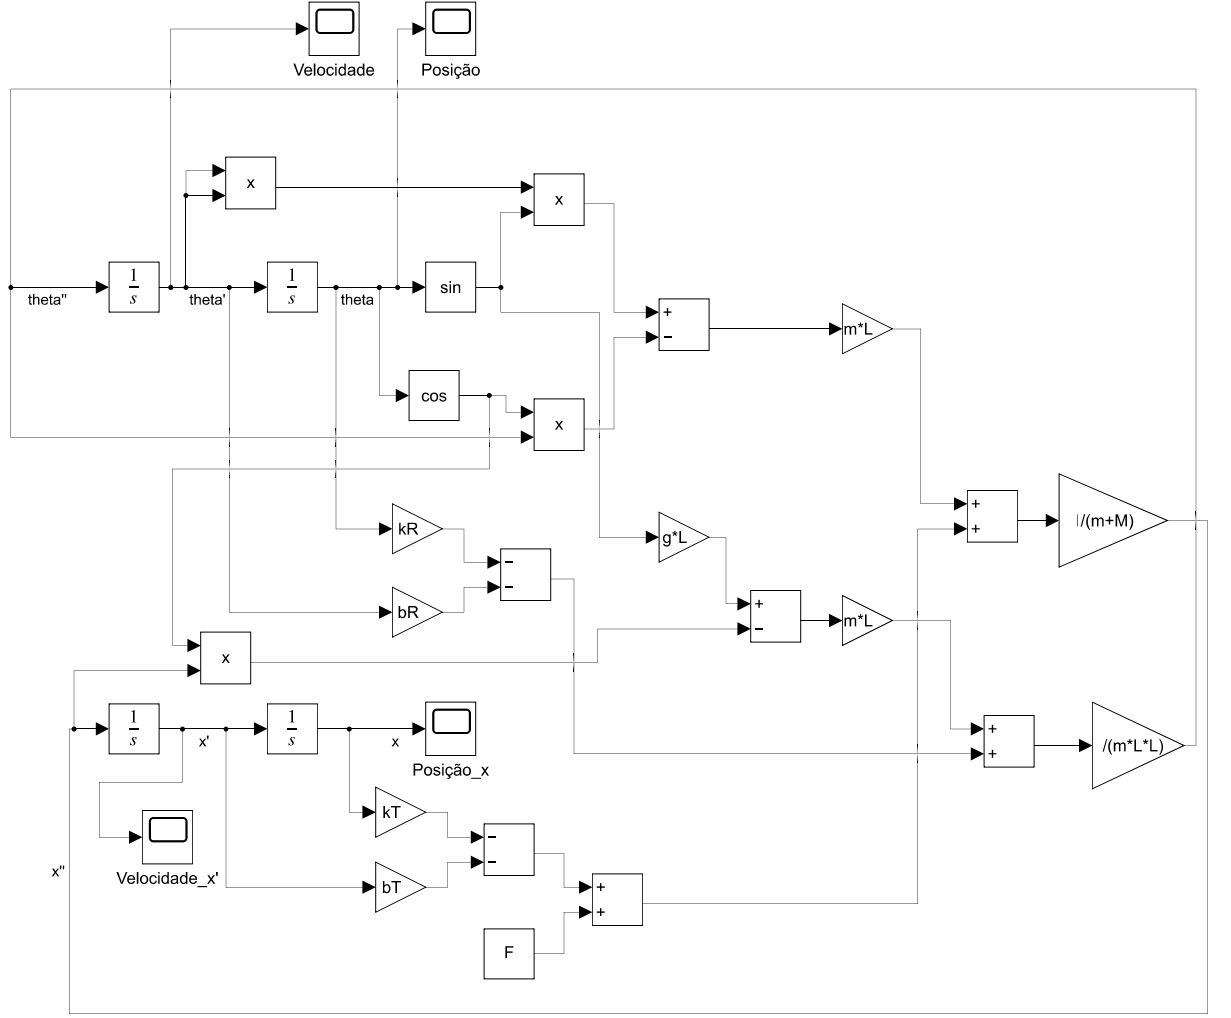
\includegraphics[scale = 0.6]{images/simulink.png}
\label{filtro1}
\caption{Modelagem do sistema no Simulink}
\end{figure}



\subsection{Resposta Dinâmica do Sistema - Simscape Multibody}

Encontramos a resposta dinâmica do sistema usando o Simscape Multibody, com os mesmos parâmetros do item anterior. A modelagem realizada é representada pela imagem abaixo:

\begin{figure}[H]
\centering
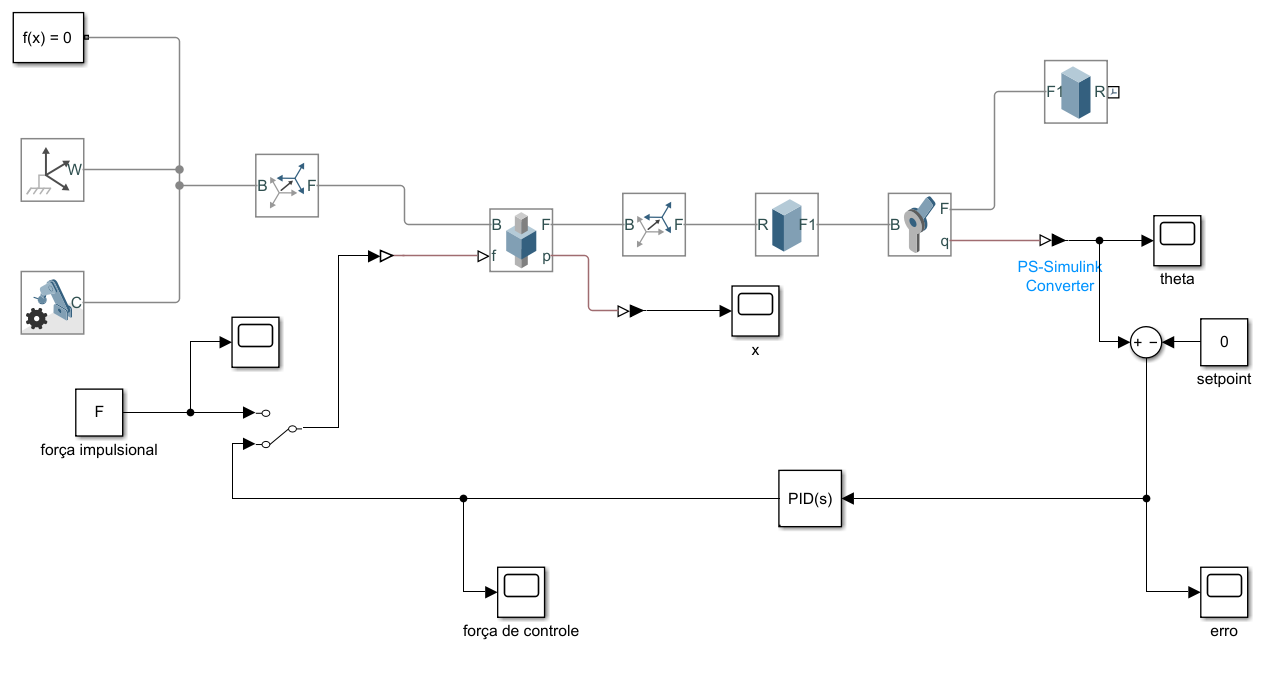
\includegraphics[scale = 0.6]{images/simscape_multibody.png}
\label{filtro1}
\caption{Modelagem do sistema no Simscape Multibody}
\end{figure}

\begin{figure}[H]
\centering
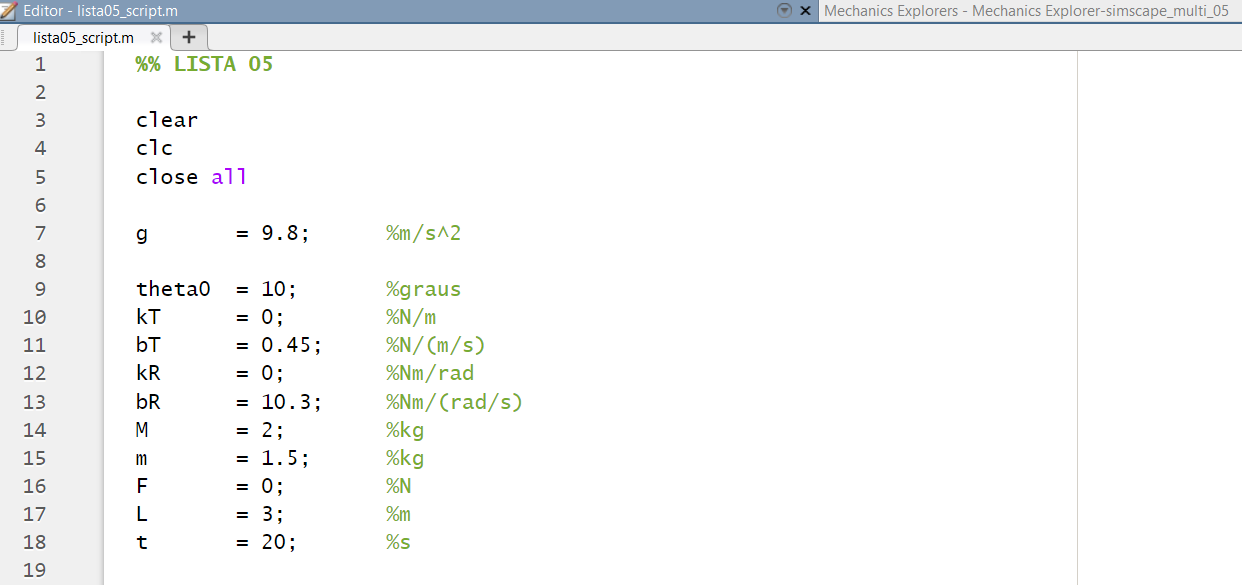
\includegraphics[scale = 0.6]{images/script_sims_multi.png}
\label{filtro1}
\caption{Script compilado em paralelo com a modelagem}
\end{figure}




\subsection{Definição dos Parâmetros}

Criamos um script no MATLAB para definir os parâmetros do sistema e rodar os dois modelos
(Simulink e Simscape).


\begin{figure}[H]
\centering
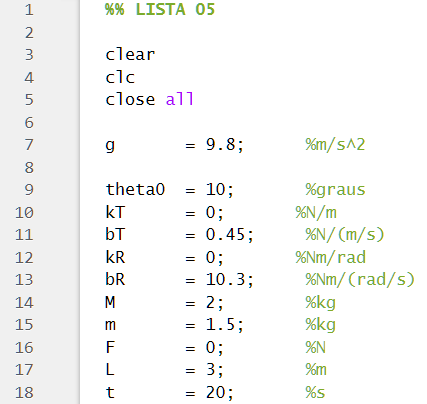
\includegraphics[scale = 0.7]{images/script.png}
\label{filtro1}
\caption{Script no MATLAB para compilar em paralelo com as modelagens.}
\end{figure}


\subsection{Respostas Gráficas}

No script criado, geramos os gráficos de posição/velocidade do carro e ângulo da haste em função do tempo. Enviamos a resposta do Simulink para o workspace do MATLAB e plotamos no script.

Com os parâmetros determinados e a condição inicial inserida, obtivemos os seguintes resultados gráficos:

\begin{figure}[H]
\centering
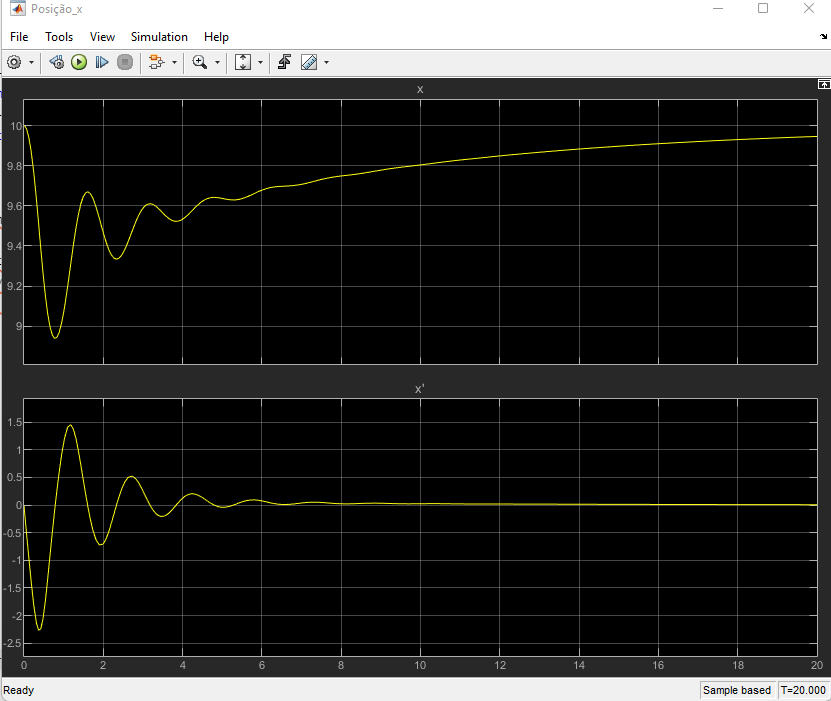
\includegraphics[scale = 0.6]{images/x_pos_vel.png}
\label{filtro1}
\caption{Gráficos gerados pelo Simulink - Posição/velocidade para x}
\end{figure}

\begin{figure}[H]
\centering
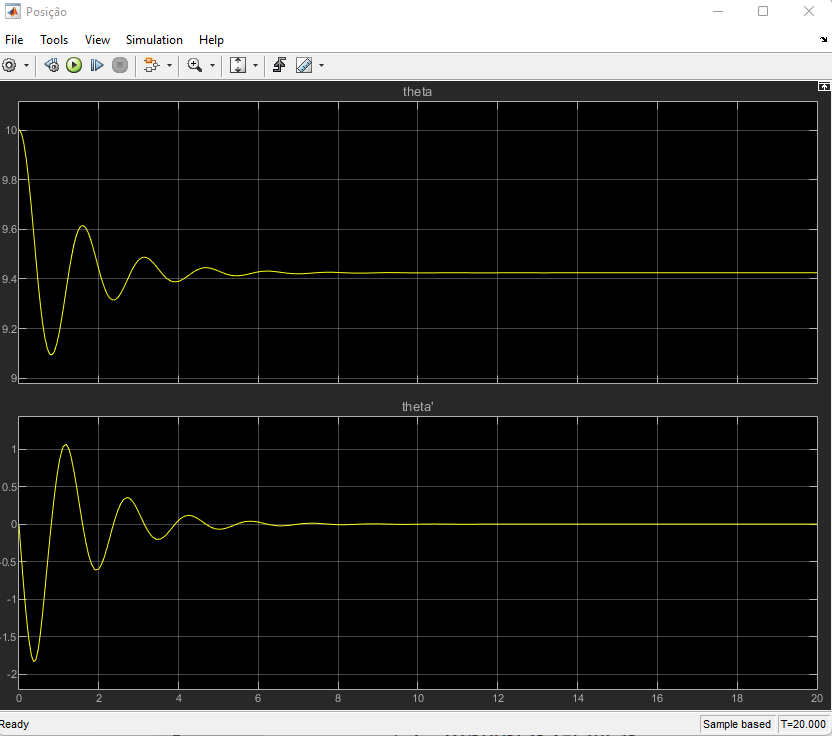
\includegraphics[scale = 0.6]{images/theta_pos_vel.png}
\label{filtro1}
\caption{Gráficos gerados pelo Simulink - Posição/velocidade para theta}
\end{figure}

\subsection{Análise do Funcionamento do Sistema}
%Explique o comportamento do sistema. Compare os resultados obtidos no Simulink e no Simscape Multibody;
Através das análises gráficas, podemos perceber o comportamento de um sistema amortecido de um carro com uma haste que pode se deslocar angularmente. A haste tende a cair sob efeito da gravidade, portanto é um sistema naturalmente instável. O sistema pode ser estabilizado aplicando uma força horizontal ao carrinho, fazendo a haste ficar na vertical. O sistema tem como entrada a força $F$, que move o carro horizontalmente e, como saídas, a posição angular do pêndulo $\theta$ e a posição horizontal do carro $x$.  A técnica utilizada para gerar o equilíbrio necessário para o pêndulo invertido é baseada no ângulo.

Analisando os gráficos gerados no Simscape, por exemplo, podemos ver que o erro começa com um valor que é proporcional à diferença entre $theta0$ e $zero$ e vai se estabilizando depois, indo para um valor nulo. Se aumentarmos o $theta0$, o valor inicial do ângulo torna-se maior e, ainda assim, o sistema consegue equilibrar até um determinado valor limite (quando testamos com $theta0 = 180rad$, por exemplo, o carro já não conseguia colocar a haste em equilíbrio).

\begin{figure}[H]
\centering
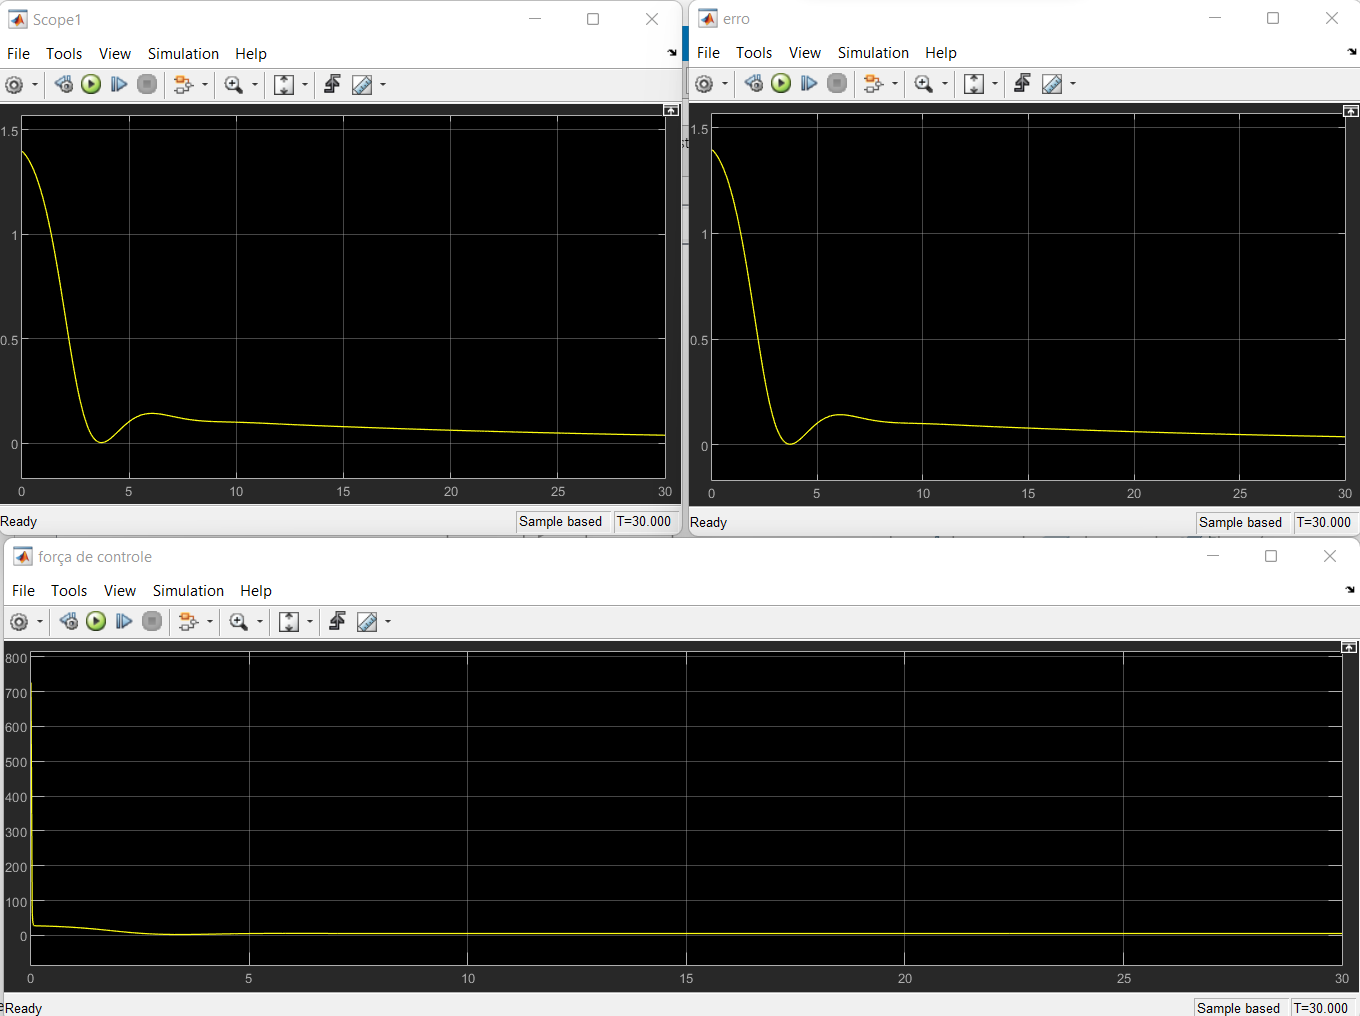
\includegraphics[scale = 0.50]{images/graficos_simscape.png}
\label{filtro1}
\caption{Gráficos gerados com a simulação no Simscape Multibody}
\end{figure}


Se compararmos as duas modelages, Simulink e Simscape, podemos verificar uma semelhança no comportamento e nas respostas gráficas, pois ambas fazem sentido e se complementam, uma vez que esperamos que a posição do carro e do ângulo comecem com uma "perturbação" para ir se estabilizando e tendendo à zero, como podemos verificar nos gráficos com o Simulink. Nos gráficos gerados pelo Simscape, verificamos que a ação proporcional, integral e derivativa atua no erro de forma a estabilizá-lo e diminui-lo, o mesmo acontece com a força. Isso faz com que o carro e a haste tendam à inercia.



\subsection{Redefinição dos Parâmetros - Repouso da Haste < 5 s}
Redefinimos os parâmetros para que a haste fique em repouso em menos de 5 segundos. %Explique a escolha de parâmetros e plote os resultados no script.

Para esta etapa, modificamos os parâmetros de forma a manter o coeficiente de amortecimento rotacional, $bR$ maior, seguida da constante de atrito $kR$, tornando o movimento do pêndulo mais rígido e aproximando-o do estado de repouso em menos tempo.


\begin{figure}[H]
\centering
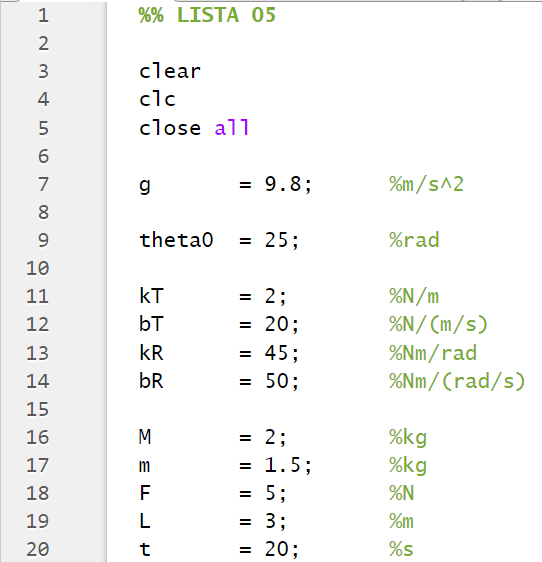
\includegraphics[scale = 0.7]{images/menos_de_5sec_script.png}
\label{filtro1}
\caption{Q.07 - Script}
\end{figure}

\begin{figure}[H]
\centering
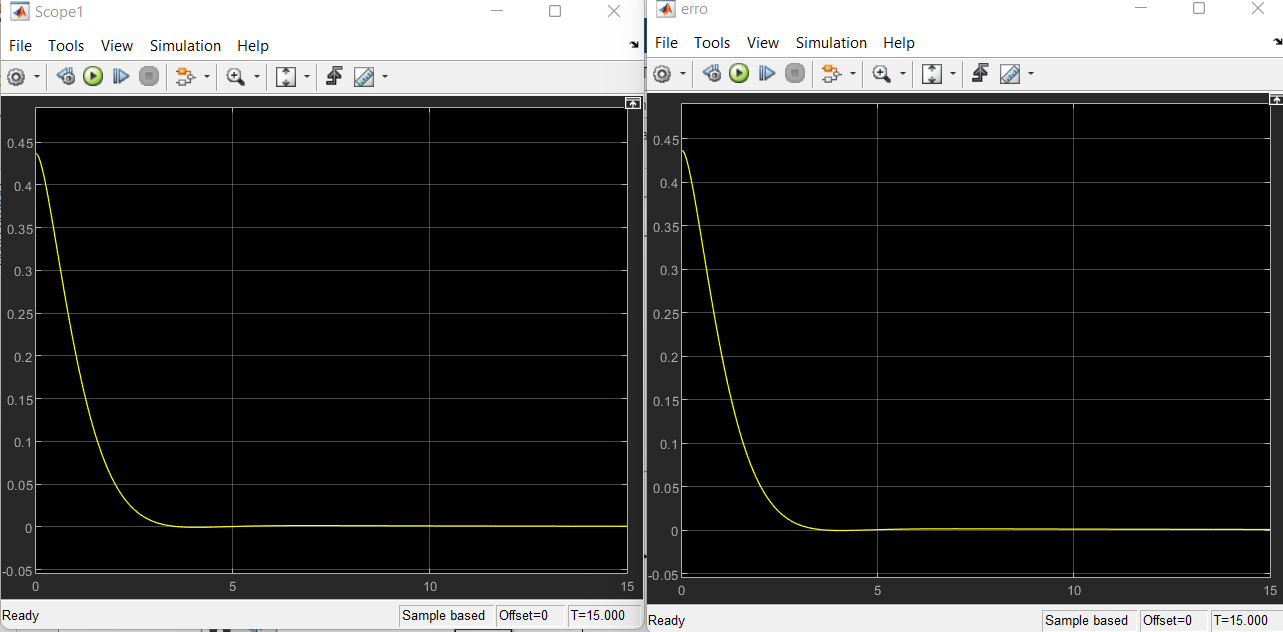
\includegraphics[scale = 0.6]{images/menos_de_5_sec_graph_sims.png}
\label{filtro1}
\caption{Q.07 - Gráficos referentes ao ângulo e ao erro, respectivamente}
\end{figure}

\begin{figure}[H]
\centering
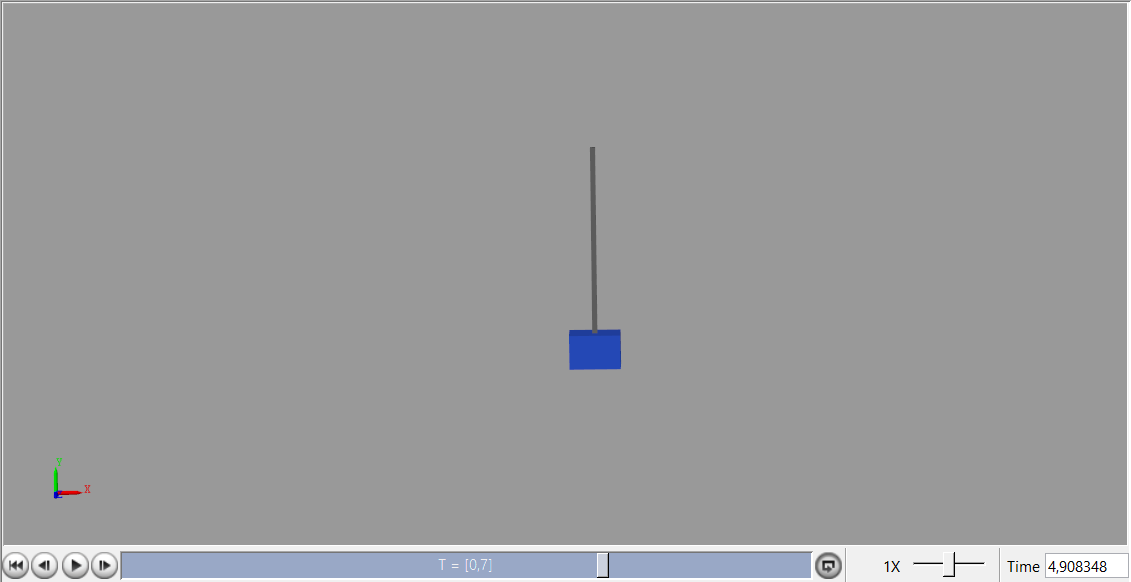
\includegraphics[scale = 0.6]{images/menos_de_5_sec.png}
\label{filtro1}
\caption{Animação Simscape - pêndulo se estabilizando em menos de 5 segundos}
\end{figure}





\subsection{Redefinição dos Parâmetros - Repouso da Haste < 10 s}
Redefinimos os parâmetros para que a haste fique em repouso em menos de 10 segundos. %Explique a escolha de parâmetros e plote os resultados no script.
\begin{figure}[H]
\centering
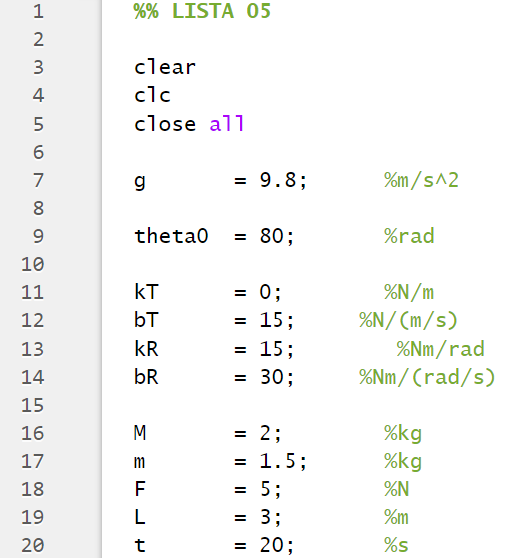
\includegraphics[scale = 0.7]{images/menos_de_10_sec_script.png}
\label{filtro1}
\caption{Q.08 - Script}
\end{figure}

\begin{figure}[H]
\centering
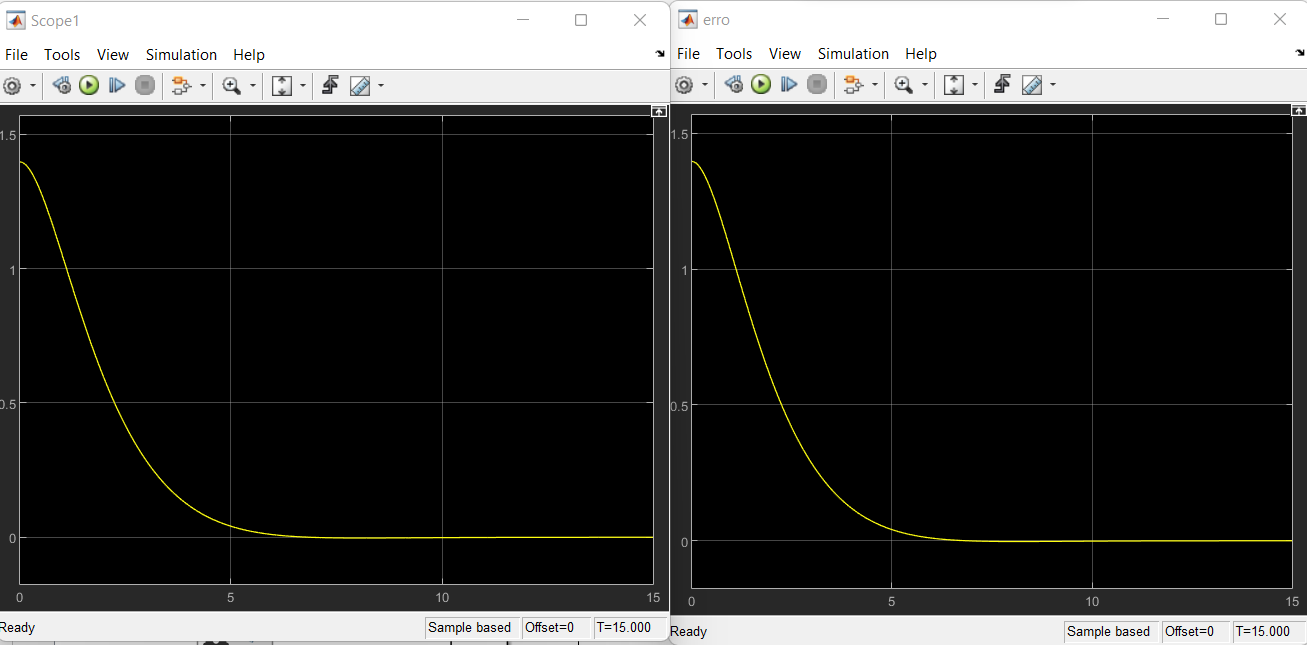
\includegraphics[scale = 0.6]{images/menos_de_10_sec_graph_sims.png}
\label{filtro1}
\caption{Q.08 - Gráficos posição/velocidade gerados com a simulação no Simulink}
\end{figure}

\begin{figure}[H]
\centering
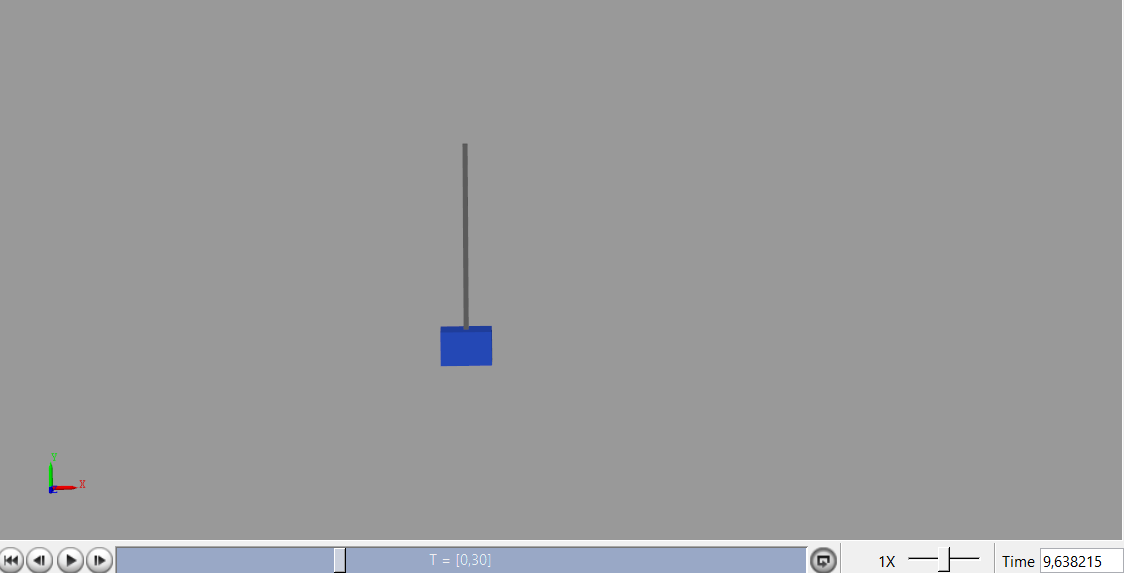
\includegraphics[scale = 0.6]{images/menos_de_10_sec.png}
\label{filtro1}
\caption{Animação Simscape - pêndulo se estabilizando em menos de 10 segundos}
\end{figure}



\subsection{Redefinição dos Parâmetros - Comportamento Estável}
Fizemos a redefinição dos parâmetros para que o sistema se comporte como um pêndulo simples de base estática. Testamos com $\theta_0 = 30 \>\ graus$. %Explique a escolha de parâmetros e plote os resultados no script.

\begin{figure}[H]
\centering
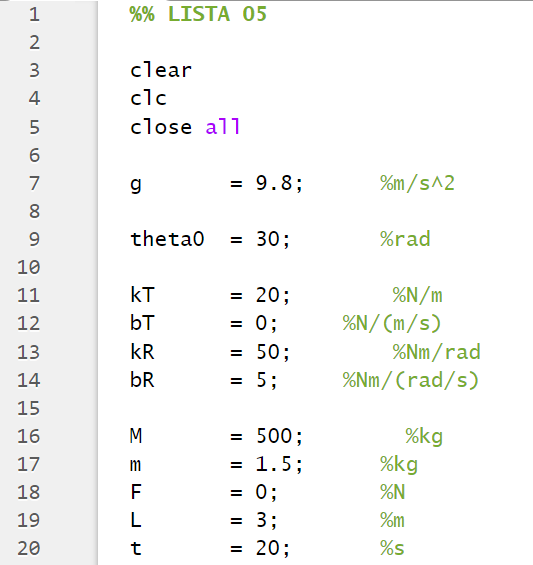
\includegraphics[scale = 0.6]{images/09_script.png}
\label{filtro1}
\caption{Q. 09 - Script}
\end{figure}


\begin{figure}[H]
\centering
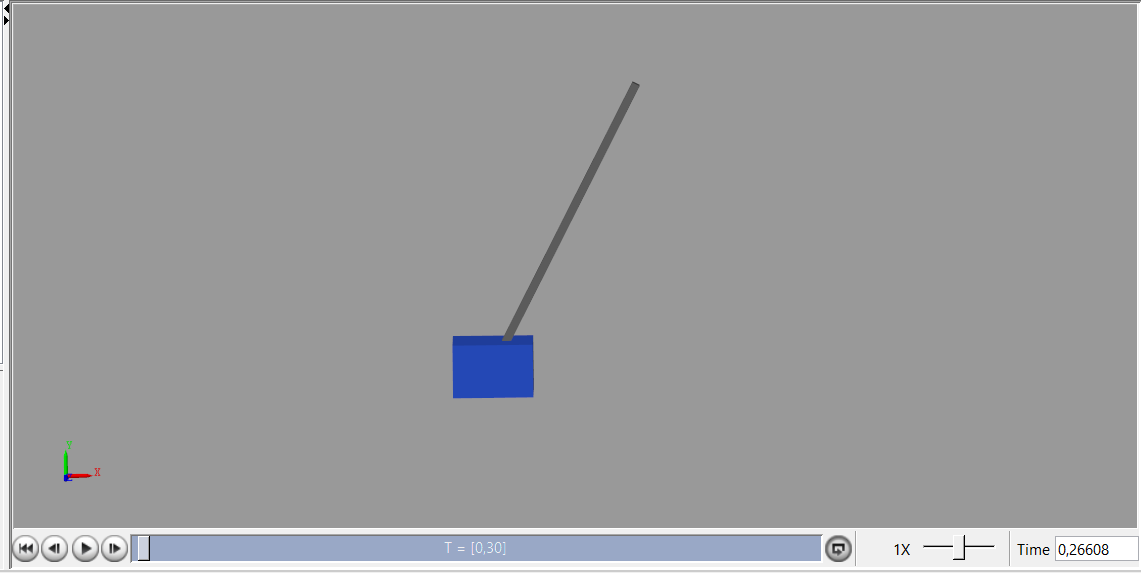
\includegraphics[scale = 0.6]{images/09_pend_ini.png}
\label{filtro1}
\caption{Q. 09 - Posição inicial do pêndulo}
\end{figure}

\begin{figure}[H]
\centering
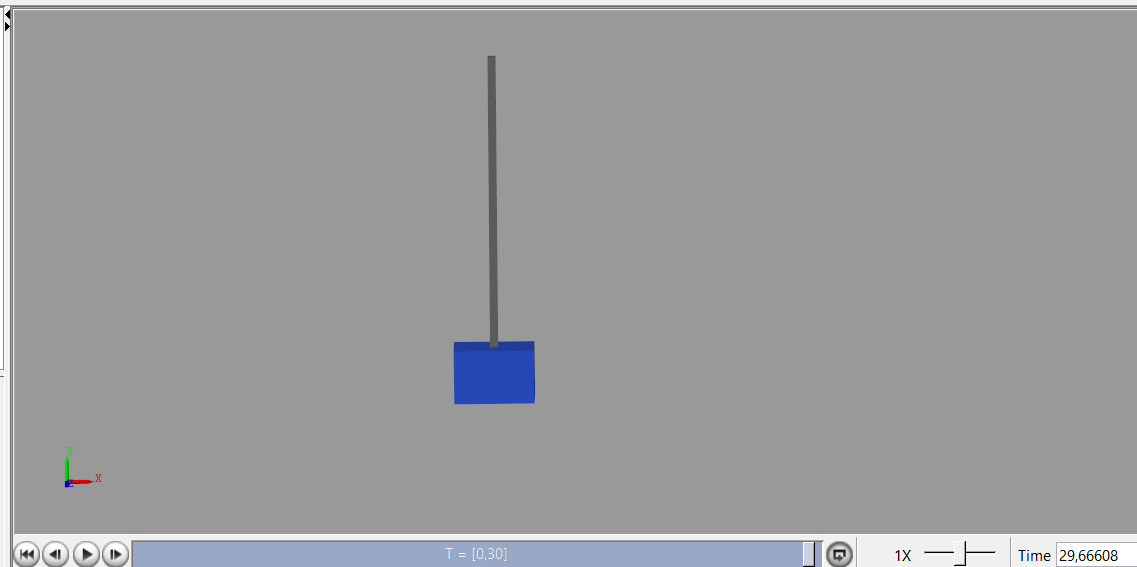
\includegraphics[scale = 0.6]{images/09_pend_final.png}
\label{filtro1}
\caption{Q. 09 - Posição inicial do pêndulo (carro inerte)}
\end{figure}

\begin{figure}[H]
\centering
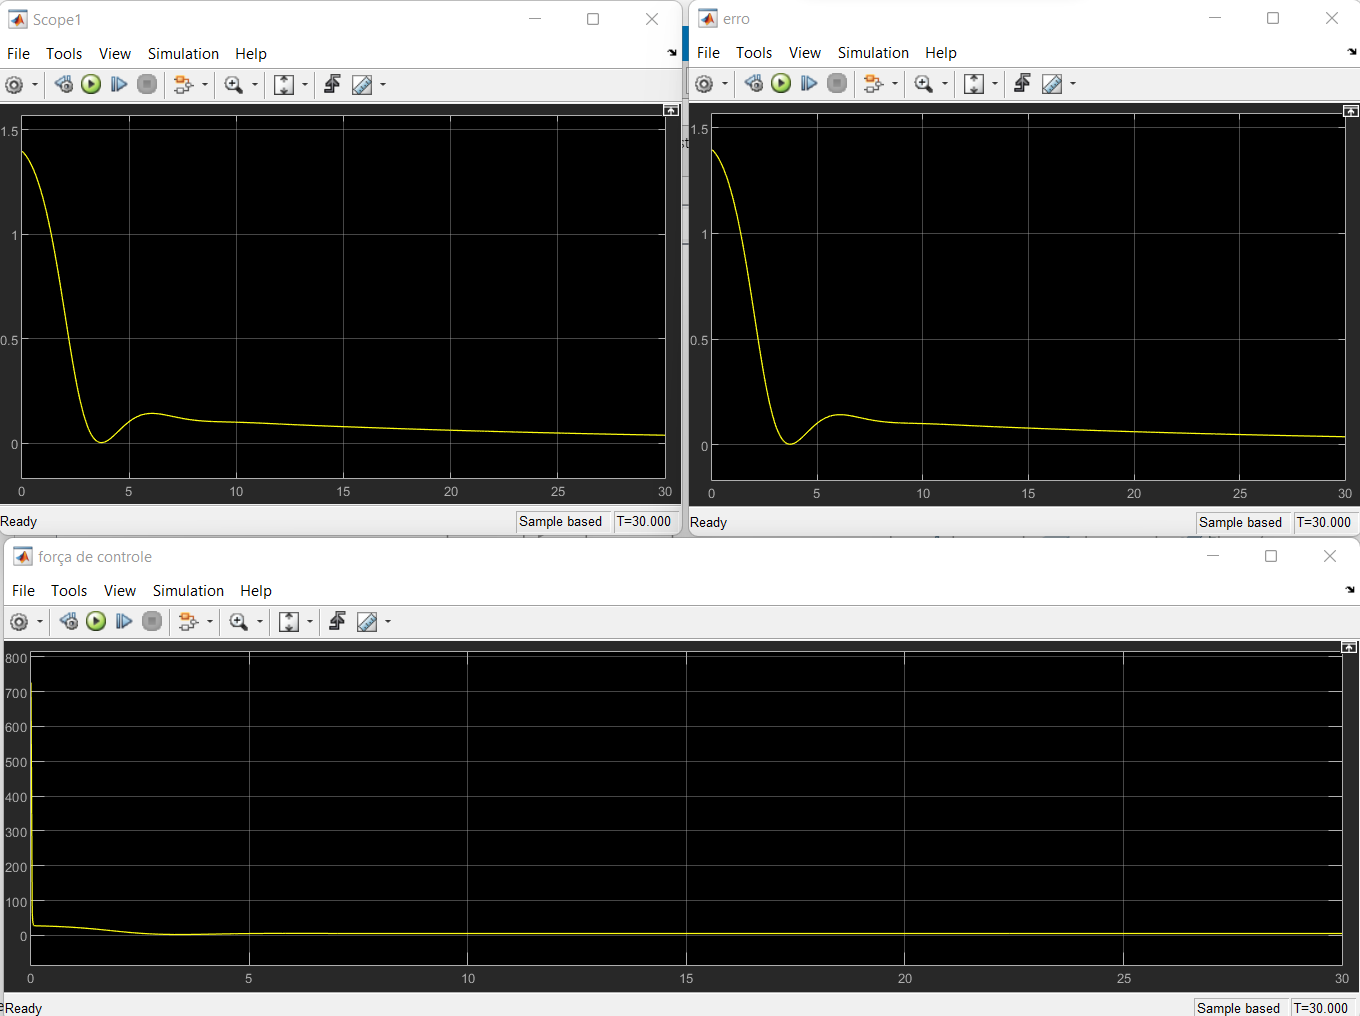
\includegraphics[scale = 0.6]{images/graficos_simscape.png}
\label{filtro1}
\caption{Q. 09 - Posição final do pêndulo (carro inerte)}
\end{figure}

\begin{figure}[H]
\centering
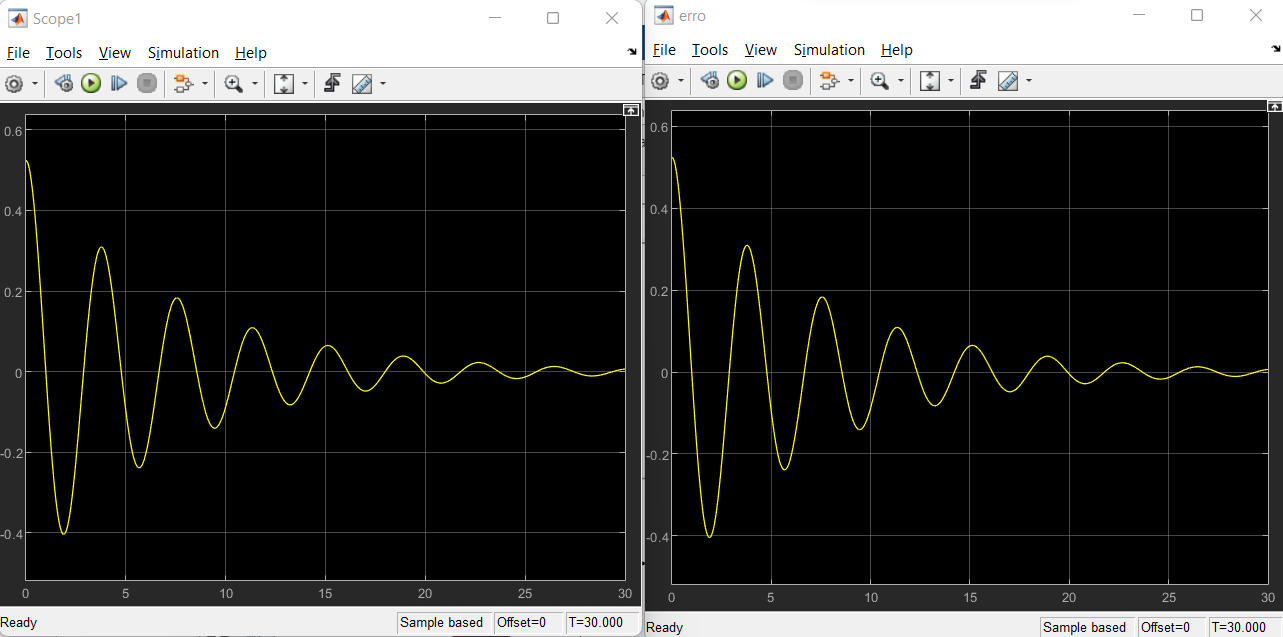
\includegraphics[scale = 0.6]{images/09_graph.png}
\label{filtro1}
\caption{Gráfico da resposta devida ao comportamento estável (pêndulo simples de base estática)}
\end{figure}



\subsection{Redefinição dos Parâmetros - Sistema massa-mola-amortecedor}
Redefinimos os parâmetros para que o sistema se comporte como um sistema massa-mola-amortecedor puramente oscilatório. Testamos com uma força $F$ não-nula. %Explique a escolha de parâmetros e plote os resultados no script.

\begin{figure}[H]
\centering
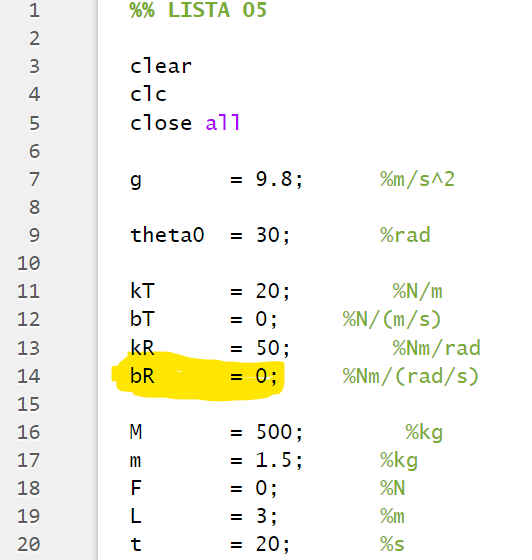
\includegraphics[scale = 0.6]{images/10_script.png}
\label{filtro1}
\caption{Q. 10 - Script}
\end{figure}


\begin{figure}[H]
\centering
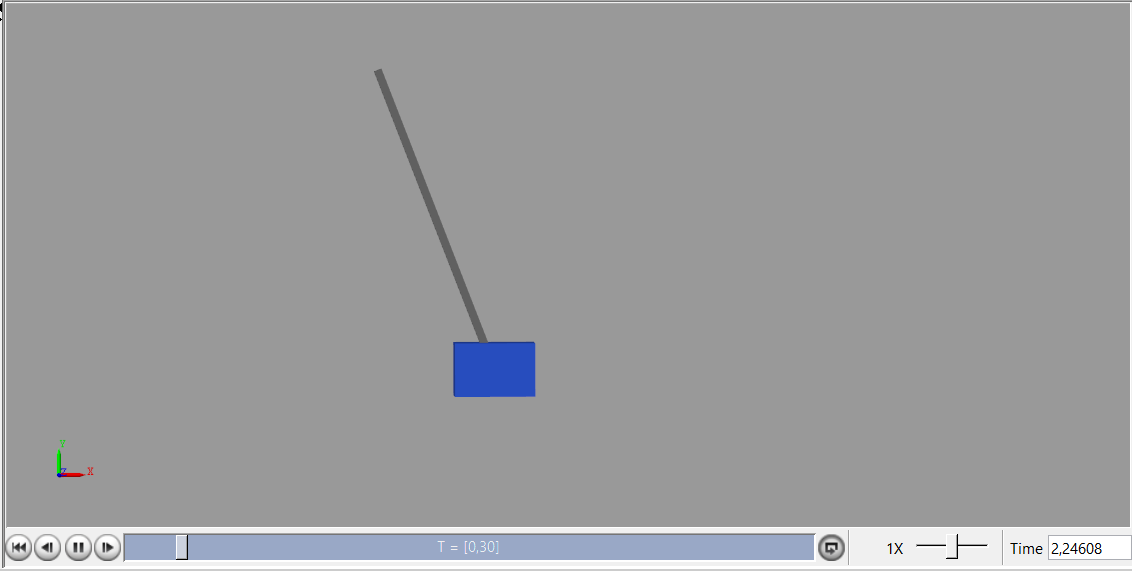
\includegraphics[scale = 0.6]{images/pend_10_ini.png}
\label{filtro1}
\caption{Q. 10 - Posição inicial do pêndulo}
\end{figure}

\begin{figure}[H]
\centering
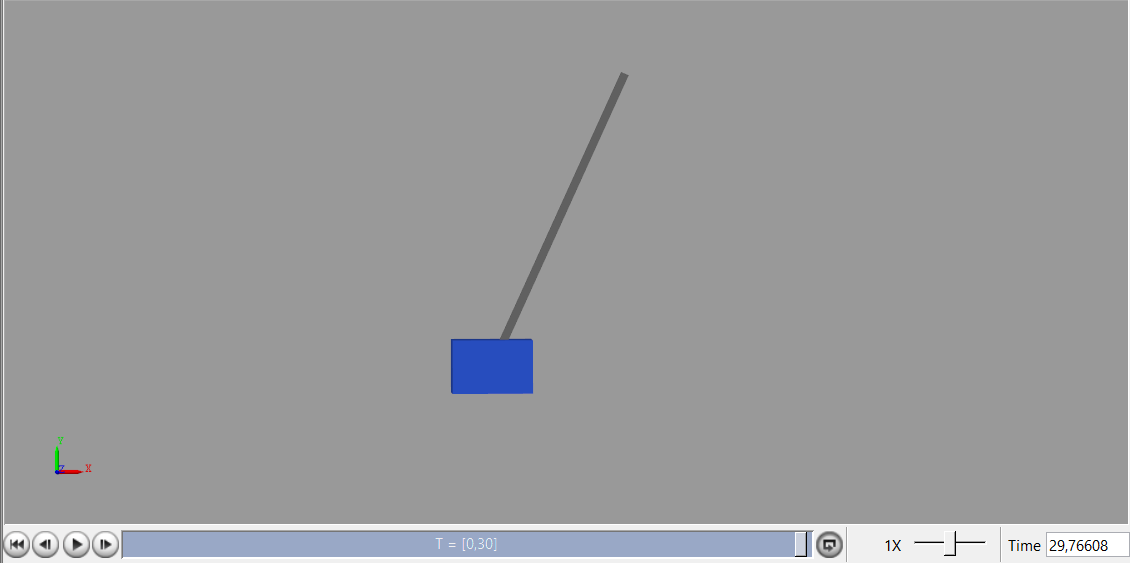
\includegraphics[scale = 0.6]{images/10_final.png}
\label{filtro1}
\caption{Q. 10 - Posição final do pêndulo}
\end{figure}

\begin{figure}[H]
\centering
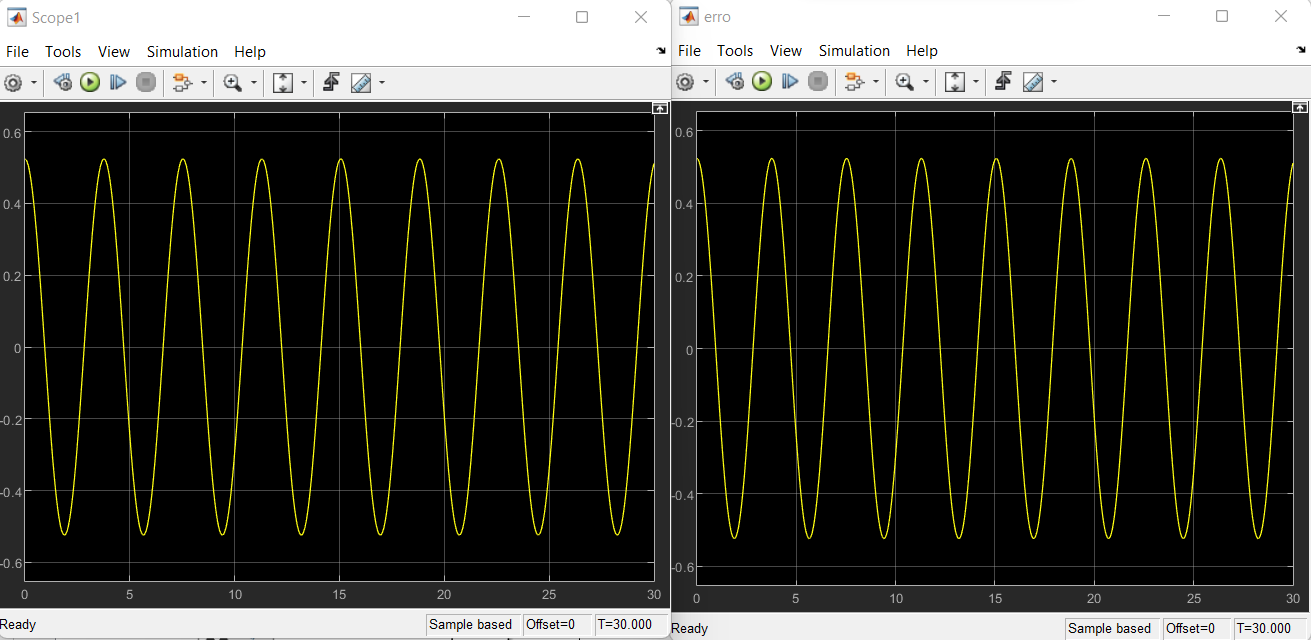
\includegraphics[scale = 0.6]{images/10_graph.png}
\label{filtro1}
\caption{Resposta gráfica do comportamento puramene oscilatório}
\end{figure}



\newpage
% REFERENCIAS %%%%%%%%%%%%%%%%%%%%%%%%%%%%%%%%%%%%%%%%%%%%%%%%%%%%%%%%%%%%%%
    \nocite{*}
    \bibliography{src/bibliography}
    
\end{document}
\section{Referências Bibliográficas}



\end{document}